\documentclass[a4paper,
fontsize=11pt,
%headings=small,
oneside,
numbers=noperiodatend,
parskip=half-,
bibliography=totoc,
final
]{scrartcl}

\usepackage[babel]{csquotes}
\usepackage{synttree}
\usepackage{graphicx}
\setkeys{Gin}{width=.4\textwidth} %default pics size

\graphicspath{{./plots/}}
\usepackage[ngerman]{babel}
\usepackage[T1]{fontenc}
%\usepackage{amsmath}
\usepackage[utf8x]{inputenc}
\usepackage[hyphens]{url}
\usepackage{xurl}
\usepackage{booktabs} 
\usepackage[left=2.4cm,right=2.4cm,top=2.3cm,bottom=2cm,includeheadfoot]{geometry}
\usepackage{eurosym}
\usepackage{multirow}
\usepackage[ngerman]{varioref}
\setcapindent{1em}
\renewcommand{\labelitemi}{--}
\usepackage{paralist}
\usepackage{pdfpages}
\usepackage{lscape}
\usepackage{float}
\usepackage{acronym}
\usepackage{eurosym}
\usepackage{longtable,lscape}
\usepackage{mathpazo}
\usepackage[normalem]{ulem} %emphasize weiterhin kursiv
\usepackage[flushmargin,ragged]{footmisc} % left align footnote
\usepackage{ccicons} 
\setcapindent{0pt} % no indentation in captions

%%%% fancy LIBREAS URL color 
\usepackage{xcolor}
\definecolor{libreas}{RGB}{112,0,0}

\usepackage{listings}

\urlstyle{same}  % don't use monospace font for urls

\usepackage[fleqn]{amsmath}

%adjust fontsize for part

\usepackage{sectsty}
\partfont{\large}

%Das BibTeX-Zeichen mit \BibTeX setzen:
\def\symbol#1{\char #1\relax}
\def\bsl{{\tt\symbol{'134}}}
\def\BibTeX{{\rm B\kern-.05em{\sc i\kern-.025em b}\kern-.08em
    T\kern-.1667em\lower.7ex\hbox{E}\kern-.125emX}}

\usepackage{fancyhdr}
\fancyhf{}
\pagestyle{fancyplain}
\fancyhead[R]{\thepage}

% make sure bookmarks are created eventough sections are not numbered!
% uncommend if sections are numbered (bookmarks created by default)
\makeatletter
\renewcommand\@seccntformat[1]{}
\makeatother

% typo setup
\clubpenalty = 10000
\widowpenalty = 10000
\displaywidowpenalty = 10000

\usepackage{hyperxmp}
\usepackage[colorlinks, linkcolor=black,citecolor=black, urlcolor=libreas,
breaklinks= true,bookmarks=true,bookmarksopen=true]{hyperref}
\usepackage{breakurl}

%meta
%meta

\fancyhead[L]{S. Menzel\\ %author
LIBREAS. Library Ideas, 37 (2020). % journal, issue, volume.
\href{https://doi.org/10.18452/21543}{\color{black}https://doi.org/10.18452/21543}
{}} % doi 
\fancyhead[R]{\thepage} %page number
\fancyfoot[L] {\ccLogo \ccAttribution\ \href{https://creativecommons.org/licenses/by/4.0/}{\color{black}Creative Commons BY 4.0}}  %licence
\fancyfoot[R] {ISSN: 1860-7950}

\title{\LARGE{Gibt es Teaching Librarians an Öffentlichen Bibliotheken? Stellen für die Förderung von Informationskompetenz}}% title
\author{Sina Menzel} % author

\setcounter{page}{1}

\hypersetup{%
      pdftitle={Gibt es Teaching Librarians an Öffentlichen Bibliotheken? Stellen für die Förderung von Informationskompetenz},
      pdfauthor={Sina Menzel},
      pdfcopyright={CC BY 4.0 International},
      pdfsubject={LIBREAS. Library Ideas, 37 (2020).},
      pdfkeywords={Öffentliche Bibliothek, Teaching Library, Informationskompetenz, Informationskompetenzvermittlung, Leseförderung, Sprachförderung, Berufliche Kompetenz, Stellenausschreibungen},
      pdflicenseurl={https://creativecommons.org/licenses/by/4.0/},
      pdfcontacturl={http://libreas.eu},
      baseurl={https://doi.org/10.18452/21543},
      pdflang={de},
      pdfmetalang={de}
     }



\date{}
\begin{document}

\maketitle
\thispagestyle{fancyplain} 

%abstracts
\begin{abstract}
\noindent
\textbf{Kurzfassung}: Eine Teaching Library fördert durch die
Bereitstellung von Lernraum und die aktive Lehre die
Informationskompetenz ihrer Nutzenden. Der Begriff \linebreak kommt ursprünglich
aus dem Bereich der Hochschulbibliotheken und ist im Zusammenhang mit
Öffentlichen Bibliotheken scheinbar selten gebräuchlich. Der folgende
Artikel geht den Fragen nach, ob dennoch Teaching Librarians in
Öffentlichen Bibliotheken in Deutschland gesucht und beschäftigt werden
und welche Berufskompetenzen gegebenenfalls dabei gefordert werden. Die
präsentierte Erhebung und Auswertung ist im Rahmen einer Vorstudie für
die Masterarbeit der Autorin entstanden (Menzel 2019).

\begin{center}\rule{0.5\linewidth}{0.5pt}\end{center}

\noindent\textbf{Abstract}: A Teaching Library supports users in improving their
information literacy. This includes the provision of working space and
access to information as well as teaching activities provided by so
called Teaching Librarians. The term was established by college and
research libraries. In the context of public libraries, it is rarely
used. This article examines whether Teaching Librarians are being hired
by German public libraries nonetheless, and if so, which competencies
are required for their work. The presented study was conducted as a
preliminary study to the author's master's thesis (Menzel 2019).
\end{abstract}

%body
\hypertarget{einleitung}{%
\section{Einleitung}\label{einleitung}}

Bibliotheken, egal welcher Sparte sie angehören, stellen in Deutschland
jeden Tag konsumfreien Arbeitsraum und Informationszugänge für ihre
Nutzenden bereit. Damit unterstützen sie, dass diese ihre Kompetenzen
selbstständig erweitern können. Darüber hinaus gibt es an vielen
deutschen Bibliotheken auch Veranstaltungen, bei denen durch
Bibliothekspersonal aktiv Kompetenzen bei den Nutzenden gefördert
werden, allen voran die Informationskompetenz (IK).\footnote{IK
  beinhaltet dabei vor allem die Suche, Bewertung und Nutzung von
  Information. Eine detaillierte Darlegung der Begriffsdefinition von
  Informationskompetenz kann im Rahmen dieses Beitrags nicht geleistet
  werden, vergleiche hierzu Menzel (2019), S. 15 ff.} Dies ist die
Aufgabe der Teaching Librarians.

Um den Beruf Teaching Librarian speziell im Hinblick auf Öffentliche
Bibliotheken (ÖB) zu betrachten, wird dieser Beitrag auf folgende Fragen
eingehen:

\begin{enumerate}
\def\labelenumi{\arabic{enumi}.}
\item
  Gibt es Teaching Librarians an Öffentlichen Bibliotheken?
\item
  Wenn ja, welche Berufskompetenzen werden von ihnen gefordert?
\end{enumerate}

\hypertarget{warum-sind-diese-fragen-wichtig}{%
\section{Warum sind diese Fragen
wichtig?}\label{warum-sind-diese-fragen-wichtig}}

Im wissenschaftlichen Diskurs zur Informationskompetenz sind selten
Stimmen aus Öffentlichen Bibliotheken zu vernehmen. Dies gilt nicht nur
für Deutschland, sondern auch international. Eine szientometrische
Analyse des Forschungsfeldes aus dem Jahr 2016 ergab beispielsweise,
dass IK-Publikationen im Zusammenhang mit Bibliotheken quasi
ausschließlich auf Wissenschaftliche Bibliotheken (WB) Bezug
nehmen.\footnote{Vergleiche Jaklitsch (2016), S. 37.} Eine Auswertung
aus dem Jahr 2005 zeigte darüber hinaus bereits, dass in der
einschlägigen internationalen Bibliografie \emph{Library Instruction and
Information Literacy} der Publikationsanteil mit Bezug auf Öffentliche
Bibliotheken von Beginn 1973 bis 2003 lediglich zwischen 1,5 \% und
2\,\% lag.\footnote{Vergleiche Ingold (2005), S. 20--21}

Gleichzeitig haben Ergebnisse der letzten zwei Jahrzehnte aus Studien
wie PISA, ICILS und IGLU\footnote{PISA: Programme for International
  Student Assessment; ICILS: International Computer and Information
  Literacy Study; IGLU: Internationale Grundschul-Lese-Untersuchung.}
dafür gesorgt, dass die Notwendigkeit von Informationskompetenzförderung
durch Bildungsinstitutionen international anerkannt wurde.\footnote{Vergleiche
  Europäische Union (2000).} Insbesondere der Stellenwert von
Bibliotheken wird dabei immer wieder betont. Die Proband\_innen der
Studien, Schüler\_innen verschiedenen Alters, sind dabei vor allem in
den Zielgruppen Öffentlicher Bibliotheken zu verorten.

Informationskompetenz soll also von Bibliotheken gefördert werden.
Konsens fehlt allerdings bei der Frage, was genau
Informationskompetenzförderung überhaupt beinhaltet. Dass sie aber in
Wissenschaftlichen Bibliotheken stattfindet -- allen voran den
Hochschulbibliotheken -- scheint allein schon durch die Gremienarbeit
deutlich: Die gemeinsame \emph{Kommission Informationskompetenz} des
Deutschen Bibliotheksverbandes (dbv) und des Vereins Deutscher
Bibliothekarinnen und Bibliothekare (VDB) beispielsweise hat derzeit
unter den sechs Mitgliedern fünf aus WB und ein Mitglied aus dem
Ausbildungsbereich.\footnote{Vergleiche IK-Kommission (2020).}
Öffentliche Bibliotheken fehlen hier. Sie sind vertreten in anderen
Kommissionen des dbv, zum Beispiel \emph{Bibliothek und Schule} oder
\emph{Kinder- und Jugendbibliotheken}. Dazu Sühl-Strohmenger:

\begin{quote}
\enquote{Die Kooperation zwischen Öffentlichen Bibliotheken und
Wissenschaftlichen Bibliotheken im Hinblick auf ihren Beitrag zum
Bildungswesen ist in Deutschland noch schwach ausgeprägt. So existieren
mit der dbv-Kommission Bildung {[}sic{]} und Schule sowie der
Gemeinsamen IK-Kommission von VDB und dbv zwei Gremien nebeneinander
ohne erkennbare Zusammenarbeit.}\footnote{Sühl-Strohmenger 2018, S. 64.}
\end{quote}

Bereits 2004 behandelten Lux und Sühl-Strohmenger das Thema Teaching
Library in Deutschland erstmals in einer eigenen Monografie, die sich
als Standardwerk etablierte\footnote{Vergleiche Simon 2007, S. 11.}.
Besonders wird hier die Spartenunabhängigkeit des Konzepts der Teaching
Library betont. Für Öffentliche Bibliotheken wird als zentraler Punkt
das \enquote{deutlich breitere Spektrum an Zielgruppen}
hervorgehoben\footnote{Lux/Sühl-Strohmenger 2004, S. 181.}. Jedoch
werden Öffentliche und Wissenschaftliche Bibliotheken insgesamt in
separaten Kapiteln behandelt; der größere inhaltliche Umfang gebührt
dabei den Hochschulbibliotheken. Ein Indiz dafür, dass sich die
IK-Arbeit in den Sparten doch signifikant unterscheidet?

Auf jeden Fall wird deutlich, dass die Arbeit, die an Öffentlichen
Bibliotheken tagtäglich geleistet wird, ebenfalls die Förderung von
Informationskompetenz beinhaltet. Dies gilt nicht trotz, sondern gerade
aufgrund der Zielgruppenvielfalt. Gut illustriert wird das durch
folgenden Ansatz von Gapski und Tekster:

\enquote{{[}O{]}hne einen ausreichenden Sprachschatz und eine
entwickelte Lesefähigkeit wird auch das Suchen und Selektieren von
Informationen zum Problem.} \footnote{Gapski/Tekster 2009, S. 57.}

Die Konsequenz dieses Zitats von Gapski und Tekster: Leseförderung und
Sprachförderung sind Förderung von Informationskompetenz. Dies belegen
auch verschiedene Modelle zur Bildung von IK. Sprachkenntnisse sowie
Lesen und Schreiben sind elementare Voraussetzungen, um kompetent mit
Information umzugehen; daher führen Maßnahmen, die das Lesen und
Schreiben fördern, mittelbar auch zu Informationskompetenz. In
Öffentlichen Bibliotheken gibt es also dann Teaching Librarians, wenn es
dort Fachkräfte gibt, die Aufgaben aus den Bereichen Lese-, Sprach- oder
IK-Förderung übernehmen.

\hypertarget{datenerhebung}{%
\section{Datenerhebung}\label{datenerhebung}}

Welche Fachkräfte von Öffentlichen Bibliotheken gesucht und beschäftigt
werden, zeigt sich wiederum in deren Stellenausschreibungen. Um die
erste Frage zu beantworten, wurden daher von Öffentlichen Bibliotheken
ausgehende Ausschreibungen ausgewertet. Da zu diesem Zweck
Ausschreibungen rückblickend betrachtet werden mussten, kamen nur
Datenquellen infrage, die eine nachträgliche Einsicht der
Ausschreibungstexte zuließen. Hier boten sich vor allem Mailinglisten
an, deren Mails in jeweils eigenen Archiven retrospektiv eingesehen
werden konnten. Dabei wurden drei einschlägige Mailinglisten betrachtet:

\begin{itemize}
\item
  \emph{ForumÖB} gibt es seit 1995. Es ist eine Mailingliste speziell
  für die Belange Öffentlicher Bibliotheken, die aus dem
  Hochschulzentrum Nordrhein-Westfalen hervorgegangen ist. Die
  Listenverantwortlichen bitten inzwischen darum, von der Verteilung von
  Stellenanzeigen über die Liste abzusehen.\footnote{Vergleiche
    Hochschulzentrum Nordrhein-Westfalen (o.\,J.).}
\item
  \emph{InetBib} ist mit 9400 (Stand März 2019) eingetragenen
  Mailadressen eine der größten Mailinglisten im Bibliotheks-, Archiv-
  und Dokumentationswesen und existiert seit 1994. Sie wurde durch die
  Universitätsbibliothek Dortmund initiiert. Ursprüngliches Thema war
  die Etablierung des Internets in Bibliotheken, daher der Listenname.
  Mittlerweile ist das Themenspektrum auf sämtliche aktuelle
  Entwicklungen im Fachbereich ausgeweitet. Darüber hinaus war
  \emph{InetBib} aufgrund der hohen Zahl an Subskribent\_innen lange
  Zeit ein viel genutzter Distributor für Stellenausschreibungen. Seit
  dem 01.04.2019 ist das Verteilen von Stellenausschreibungen über die
  Liste allerdings offiziell unerwünscht und soll auf anderen Wegen
  geschehen.\footnote{Vergleiche InetBib e.\,V. (o.\,J.).}
\item
  \emph{BAK Jobinfo} ist regional auf Informationseinrichtungen in
  Berlin und Brandenburg beschränkt. Über diese Liste werden durch den
  \emph{Berliner Arbeitskreis Information} (BAK) geprüfte
  Stellenangebote verbreitet. Die Liste hat nach Angaben des
  Arbeitskreises mehr als 2000 eingetragene Adressen.\footnote{Vergleiche
    Berliner Arbeitskreis Information (o.\,J.).}
\end{itemize}

Für die Suche nach Teaching-Librarian-Profilen in den ausgeschriebenen
Stellen wurde ein 2,5-jähriger Zeitraum von Januar 2016 bis September
2018 (Erhebungszeitpunkt) ausgewertet. Über alle drei Listen wurden in
diesem Zeitraum regelmäßig Stellenausschreibungen verschickt. In den
Listen wurden alle Nachrichten gesichtet, die von Öffentlichen
Bibliotheken ausgingen und in der Betreffzeile eine Stellenausschreibung
ankündigten. Als Öffentliche Bibliothek galten dabei der Öffentlichkeit
zugängliche Bibliotheken in öffentlicher Trägerschaft. Für die
anschließende Auswertung konnten jene Stellenanzeigen beachtet werden,
deren Tätigkeitsprofil im Text der E-Mail, durch einen funktionierenden
Link oder einen verfügbaren Anhang noch einsehbar war.

An den Daten ist zu beachten, dass bei veröffentlichten Stellenanzeigen
der Entstehungsprozess nicht nachvollziehbar und in der Regel kein\_e
Urheber\_in auszumachen ist. Darüber hinaus sind vorgefertigte
Anforderungsformulierungen durch Ankreuzsysteme oder die
Wiederverwendung von früheren Ausschreibungstexten nicht
auszuschließen.\footnote{Aus diesem Grund wurden die vorgestellten
  Ergebnisse in einer breiteren Studie in konkrete Einschätzungen und
  Beobachtungen aus dem Arbeitsalltag von Teaching Librarians an ÖB
  eingebettet, siehe hierzu Menzel (2019).} Dennoch sind es eben diese
Ausschreibungen, die über Online-Kanäle große Reichweite entfalten. Auf
diese Weise haben sie einen unmittelbaren Einfluss auf die realen
Umstände im Berufsfeld der Teaching Librarians, also die Besetzung und
Ausgestaltung der Stellen und damit die täglichen Vorgänge in
Öffentlichen Bibliotheken.

\hypertarget{vorgehen-bei-der-auswertung}{%
\section{Vorgehen bei der
Auswertung}\label{vorgehen-bei-der-auswertung}}

Eine Stelle für Teaching Librarians konnte dann festgestellt werden,
wenn in der Beschreibung des Aufgabenfeldes eine lehrende Tätigkeit in
der Bibliothek oder aber die Konzeption beziehungsweise Koordination von
Lehrangeboten im Bereich Sprach-, Lese- oder IK-Förderung beschrieben
wurde. War das der Fall, wurden die entsprechenden Nachrichten manuell
extrahiert und Dubletten aussortiert. Die Rahmenbedingungen der
Ausschreibungen wurden dabei nicht einbezogen; so wurden Voll- und
Teilzeitstellen, befristete und unbefristete Stellen (auch Krankheits-
und Elternzeitvertretungen) gleichsam beachtet. Lediglich
Ausschreibungen für Ausbildungsplätze wurden ausgeschlossen, da diese
aufgrund der Karrierestufe keine fachlichen Anforderungen stellen
konnten.

Außerdem wurde festgehalten, auf welchen Lohnstufen sich die
Ausschreibungen bewegen. Da es sich aufgrund der öffentlichen
Trägerschaft ausschließlich um tariflich bezahlte Stellen handelte,
konnten anhand der TVöD\footnote{TvÖD: Tarifvertrag Öffentlicher Dienst.}-Stufen
Rückschlüsse auf den verlangten Ausbildungsgrad gezogen werden. Die
Stufen E5--E8 wurden dabei als Stellen gewertet, die eine Ausbildung,
zum Beispiel als Fachangestellte\_r für Medien- und Informationsdienste
(FAMI), voraussetzen. Bachelor-, Diplom- oder vergleichbare Abschlüsse
wurden im Segment E9--E11 angesiedelt. Alle höheren Stufen wurden
Master-, Magister- oder vergleichbaren Abschlüssen zugeordnet.

Die Tätigkeitsbeschreibungen wurden in Codes übertragen, also
Markierungen, anhand derer die Gemeinsamkeiten über die
Stellenausschreibungen hinweg einheitlich erfasst werden konnten. Für
die Codes wurden Bezeichnungen gewählt, die das Vokabular der
Ausschreibungen direkt aufgriff. Aus diesem Grund tragen die Codes zum
Teil mehrere verwandte Bezeichnungen.\footnote{Details zum Vorgehen im
  Codierungsprozess bei Menzel (2019), S. 37.}

\hypertarget{ergebnisse}{%
\section{Ergebnisse}\label{ergebnisse}}

Insgesamt konnten 262 Ausschreibungen für Teaching Librarians ausgehend
von Öffentlichen Bibliotheken in Deutschland ausgewertet werden. Auf
diese Zahl kommt eine Dunkelziffer von 722 potenziellen Ausschreibungen,
bei denen der Volltext nicht mehr einsehbar war, die nach Betreffzeile
aber ebenfalls vermittelnde Tätigkeiten enthalten haben
könnten.\footnote{Diese Problematik trat bereits in anderen Studien mit
  Stellenausschreibungen als Datenmaterial auf, zum Beispiel bei
  Tappenbeck et al.~(2017), S. 34.} Damit konnte die erste Frage mit Ja
beantwortet werden: Teaching Librarians werden von deutschen
Öffentlichen Bibliotheken gesucht und eingesetzt.

Darüber hinaus kann für die ausgewerteten Mailinglisten ein stetiger
Anstieg an Ausschreibungen für Teaching Librarians über den untersuchten
Zeitraum festgestellt werden (vergleiche Abbildung 1).

\begin{figure}
\centering
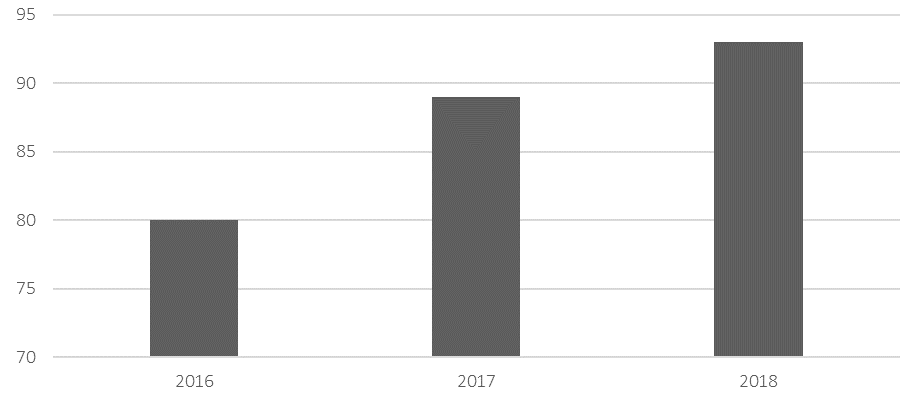
\includegraphics[width=0.8\textwidth]{img/image1.png}
\caption{Verteilung der Ausschreibungen (n=262) mit
Teaching-Librarian-Profil nach Jahren.}
\end{figure}

Unter den 262 Stellen dominieren die Vergütungsstufen, die einen
Bachelor- oder Diplomabschluss erfordern mit 70,6\,\% (185
Ausschreibungen, vergleiche Abbildung 2). Die zweitgrößte Gruppe machen
mit 22,5\,\% die Eingruppierungen für Personen mit Fachausbildung aus,
zum Beispiel Fachangestellte für Medien- und Informationsdienste aus (59
Ausschreibungen). Lediglich 2\,\% der Ausschreibungen wurden in die
Gruppen E13 oder höher eingestuft (6 Ausschreibungen).\footnote{Zum
  geringen Anteil an Stellen im oberen Vergütungssegment siehe auch
  Wimmer (2019).}

\begin{figure}
\centering

\includegraphics[width=0.8\textwidth]{img/image2.png}
\caption{Qualifikationsstufen der Ausschreibungen mit
Teaching-Librarian-Profil (n=262).}
\end{figure}

Welche Kompetenzen wurden aber im Rahmen dieser Stellen verlangt? Um
diese zweite Frage zu beantworten, war eine qualitative Datenanalyse der
Tätigkeitsprofile notwendig (vergleiche Abbildung 3). Dabei wurden die
beschriebenen Kompetenzen in insgesamt vier Gruppen eingeteilt, die sich
an den Deutschen Qualifikationsrahmen anlehnen.\footnote{BMBF 2011, S.
  5.} Sozialkompetenzen (grün) werden in der Interaktion mit anderen
eingesetzt, Selbstkompetenzen (rot) beziehen sich auf selbstbezogene
Merkmale, wie zum Beispiel Ehrgeiz. Fachkompetenzen (blau) umfassen
fachspezifische Aufgaben in einem bestimmten Arbeitsbereich und
Sachkompetenzen (gelb) spielen in verschiedenen Fachbereichen eine
Rolle, beispielsweise Sprachkenntnisse.

\begin{figure}
\centering
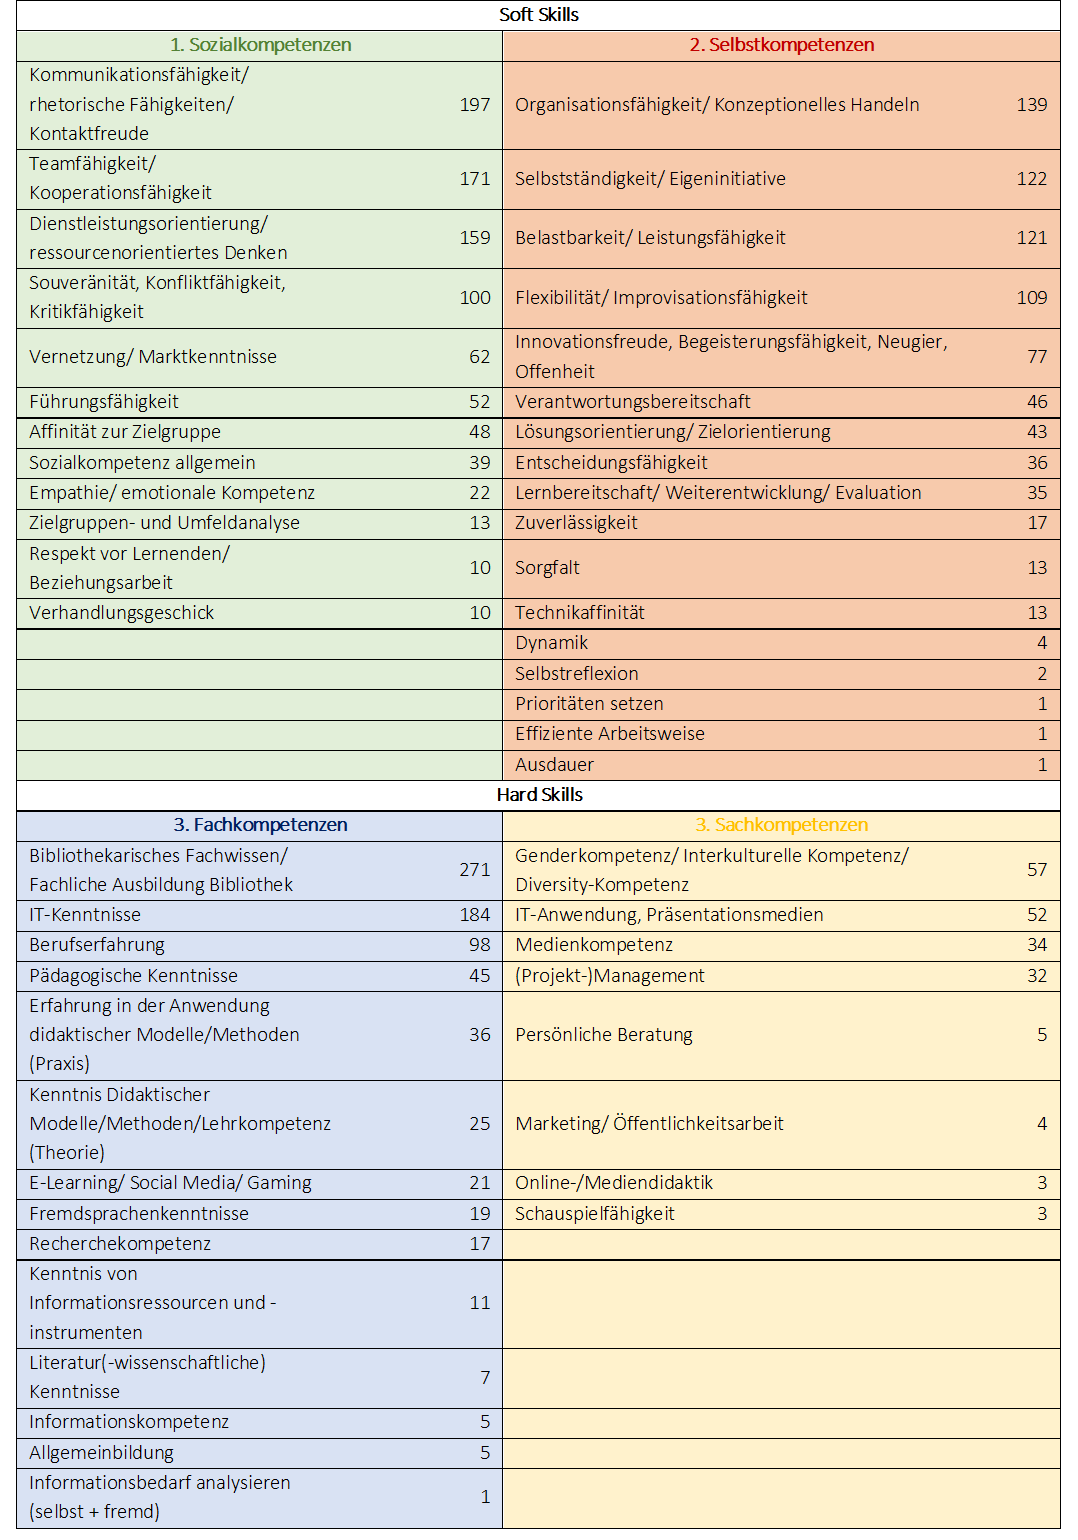
\includegraphics[width=0.9\textwidth]{img/image3.png}
\caption[Verlangte Kompetenzen im Anforderungsprofil der 265
Ausschreibungen. Anordnung absteigend nach Nennungshäufigkeit (n=262,
Mehrfachnennung derselben Kompetenz innerhalb einer Ausschreibung
möglich). Genaue Definitionen der einzelnen Kompetenzen bei Menzel
(2019), Anhang B. ]{Verlangte Kompetenzen im Anforderungsprofil der 265
Ausschreibungen. Anordnung absteigend nach Nennungshäufigkeit (n=262,
Mehrfachnennung derselben Kompetenz innerhalb einer Ausschreibung
möglich). Genaue Definitionen der einzelnen Kompetenzen bei Menzel
(2019), Anhang B. \footnotemark{}}
\end{figure}
\footnotetext{Für die vorliegende Auswertung wurden leichte Änderungen
  in der Zuordnung der Kompetenzen vorgenommen. Die ursprüngliche
  Einteilung findet sich bei Menzel (2019), Anhang A.}

Ein grundsätzliches Ergebnis in der Auswertung der Tätigkeitsprofile
ist, dass die ausgeschriebenen Stellen in den seltensten Fällen
ausschließlich Aufgaben der Lese-, Sprach- und IK-För\-derung aufwiesen.
Vielmehr handelt es sich um Stellen mit Mehrfachtätigkeit, in denen
unter anderem vermittelnde Aufgaben beinhaltet sind. Reine
Teaching-Librarian-Stellen waren kaum vorhanden. Trotz dieser
Mehrfachtätigkeit kommen die meistgeforderten Kompetenzen unmittelbar in
der Tätigkeit als Teaching Librarian zum Einsatz:

\begin{enumerate}
\def\labelenumi{\arabic{enumi}.}
\item
  Sozialkompetenzen für die \textbf{Interaktion mit
  Veranstaltungsteilnehmer\_innen}, wie Kontaktfreude,
  Kommunikationsfähigkeit und rhetorische Fähigkeiten.
\item
  Sozialkompetenzen für die \textbf{Interaktion mit Mitarbeiter\_innen},
  zum Beispiel anderen Teaching Librarians. Konkret sind das
  Teamfähigkeit und Kooperationsfähigkeit.
\item
  Selbstkompetenzen für die \textbf{Planung von Veranstaltungen}, wie
  Organisationsfähigkeit, die Fähigkeit zum konzeptionellen Denken,
  Selbstständigkeit, Eigeninitiative sowie Lösungs- und
  Zielorientierung.
\item
  Selbstkompetenzen und Sachkompetenzen für die \textbf{Durchführung von
  Veranstaltungen}, wie Flexibilität, Improvisationsfähigkeit und
  Souveränität, aber auch Wissen über den Umgang mit Diversität,
  Geschlechterrollen und Interkulturalität und über Projektmanagement.
  Einige Ausschreibungen forderten darüber hinaus die Fähigkeit, die
  Veranstaltungen durch Evaluation weiterzuentwickeln.
\item
  Fachkompetenzen für die gängigen \textbf{Abläufe in einer Bibliothek},
  wie die Kenntnis von Katalogisierungssystemen und Abläufen zur
  technischen Medienbearbeitung.
\item
  Fachkompetenzen für den \textbf{Umgang mit Informationstechnologie},
  Kenntnisse über den Umgang mit Sozialen Netzwerken,
  E-Learning-Plattformen und Gaming-Angeboten.
\item
  Fachkompetenzen zum \textbf{Erzielen optimaler Lernergebnisse in den
  Veranstaltungen}, wie die Kenntnis didaktischer Modelle und Methoden
  sowie Erfahrung in deren Anwendung.
\end{enumerate}

Darüber hinaus wurde in ungefähr einem Drittel der Ausschreibungen
Berufserfahrung gefordert (98 Codierungen in 262 Ausschreibungen).

\hypertarget{diskussion}{%
\section{Diskussion}\label{diskussion}}

Oftmals unter dem Stichwort \enquote{Paradigmenwechsel} ist in den
letzten Jahren in der Literatur immer wieder die Frage aufgekommen, ob
gerade für vermittelnde Aufgaben in Bibliotheken Personal eingestellt
werden sollte, das nicht die klassischen bibliothekarischen Ausbildungs-
und Studiengänge durchlaufen hat, sondern einen direkten Hintergrund in
der (Medien-)Didaktik und Pädagogik vorweisen kann.\footnote{Vergleiche
  Krauß-Leichert(2008), S. 7.} Ein Paradigmenwechsel kann anhand der
Ausschreibungspraxis nicht bestätigt werden. Bibliothekarische
Fachkenntnisse verschiedener Ausprägung sind omnipräsent (270
Codierungen in 262 Ausschreibungen), während pädagogische Kenntnisse
lediglich 45 Mal codiert wurden und Kenntnisse didaktischer Modelle und
Methoden lediglich 36 Mal. Denkbar ist allerdings, dass dies
vordergründig im Zusammenhang mit der Mehrfachtätigkeit steht. Ein
Großteil der Ausschreibungen beinhaltete neben der Tätigkeit als
Teaching Librarian auch Aufgaben der Erwerbung, Katalogisierung und
technischen Medienbearbeitung. Die explizite Forderung nach einer
bibliothekarischen Fachausbildung oder aber die Forderung nach genuin
bibliothekarischen Kenntnissen (zum Beispiel Katalogisierung) dominiert
damit anteilig alle anderen geforderten Kompetenzen. Bemerkenswert ist,
dass die eigene Informationskompetenz der gesuchten Person nur fünf Mal
codiert wurde. Mutmaßlich ist der kompetente Umgang mit Information also
in der Forderung nach einer bibliothekarischen Fachausbildung
eingefasst.

Über die Gründe für die Forderung von Berufserfahrung in weniger als
jeder dritten Ausschreibung lässt das Datenmaterial keine Schlüsse zu.
Eine mögliche These ist die Offenheit der ÖB gegenüber
Berufseinsteiger\_innen aufgrund der mutmaßlichen Nähe zu jüngeren
Zielgruppen. Ein weiterer denkbarer Grund ist das Potenzial, das in
einer jüngst abgeschlossenen bibliothekarischen Ausbildung im Hinblick
auf neue mediale Entwicklungen und aktuelle Veranstaltungsformate
gesehen wird. Festzuhalten ist jedenfalls, dass die ausschreibenden ÖB
die Stellen für Teaching Librarians offenbar meist auch potenziell mit
Berufseinsteiger\_innen besetzen würden.

Die aufgelisteten Hauptkompetenzen zielen unter anderem auf die
Entwicklung neuer Veranstaltungsformate ab. In diesem Zusammenhang fällt
auf, dass trotz vielfach genannter konzeptioneller Aufgaben die
Forderung nach Kreativität in keiner der Ausschreibungen vorkam.

\hypertarget{limitierungen}{%
\section{Limitierungen}\label{limitierungen}}

Nicht nur konnten die erhobenen Daten den Nachweis erbringen, dass
Teaching Librarians an ÖB eingesetzt werden, sondern auch einen Anstieg
der Stellen mit Teaching-Librarian-Profil über den untersuchten Zeitraum
aufzeigen. Dafür kann es verschiedene Gründe geben, über die die reine
Quantität der Ausschreibungen leider keine Aussage erlaubt. Denkbar
wären beispielsweise ein erhöhter Stellenwert der vermittelnden
Tätigkeiten in ÖB oder ein Generationswechsel.

Neben der bereits im Abschnitt zur Datenerhebung erwähnten Problematik
von Stellenausschreibungen als Datenquelle bilden Ausschreibungen eine
theoretische Grundlage zur Berufspraxis. Die vorliegenden Ergebnisse
lassen Schlüsse auf die Besetzungspraxis und die verlangten Kompetenzen
zu. Dies gibt die Grundlage für Aussagen darüber, wie das Berufsbild von
Teaching Librarians von ÖB in Deutschland aussieht. Es gibt aber nicht
die Grundlage für Rückschlüsse auf die tatsächliche Berufspraxis und
jene Kompetenzen, die im Arbeitsalltag von Teaching Librarians zum
Einsatz kommen.\footnote{Ergebnisse aus der Praxis bietet Menzel (2019),
  S. 47 ff.}

Das verwendete Vokabular in den Ausschreibungen wurde hier nicht
gesondert untersucht. Bemerkenswert ist jedoch, dass der Begriff
\emph{Teaching Librarian} in keiner Ausschreibung verwendet wurde. Dies
ist ein Indikator dafür, dass von WB und ÖB offenbar verschiedene
Ausdrücke für vermeintlich ähnliche Tätigkeiten verwendet wurden. Hier
wäre eine linguistische Untersuchung interessant. Darüber hinaus wäre
die genauere Untersuchung der erfassten Kompetenzen mit der
Ausschreibungspraxis Wissenschaftlicher Bibliotheken\footnote{Vergleiche
  hierzu Scholle (2016).} sinnvoll, um festzustellen, ob die Tätigkeiten
tatsächlich ähnlich beziehungsweise deckungsgleich sind. Daraus ließen
sich Konsequenzen der aktuell getrennt stattfindenden Gremienarbeit von
ÖB und WB ableiten.

Die vorliegende Auswertung nahm zwar eine Ausdifferenzierung der
Ausschreibungen nach Gehaltsstufe vor, allerdings wurden die Fähigkeiten
nicht getrennt codiert. Auch hier wäre eine weiterführende Fragestellung
wünschenswert, die geforderte Kompetenzen nach Einstufung analysiert.

\hypertarget{zusammenfassung-und-fazit}{%
\section{Zusammenfassung und
Fazit}\label{zusammenfassung-und-fazit}}

Informationskompetenzförderung fasst Sprach- und Leseförderung mit ein,
weil Sprachkenntnisse und Lesefähigkeit unmittelbare Voraussetzungen für
die kompetente Suche, Bewertung und Verarbeitung von Information sind.
In diesen Bereichen sind auch Mitarbeitende Öffentlicher Bibliotheken
tätig, als sogenannte Teaching Librarians.

Allerdings herrscht aktuell offenbar eine klare Spartentrennung zwischen
Wissenschaftlichen und Öffentlichen Bibliotheken in diesem
Tätigkeitsbereich. Das spiegelt sich unter anderem politisch wider, und
zwar in der deutschlandweiten IK-Gremienarbeit.\footnote{Eine genaue
  Ausdifferenzierung der vorhandenen Gremien nach Sparte finden Sie bei
  Menzel (2019), S. 21 ff.} Öffentliche Bibliotheken formieren sich eher
unter Ausdrücken wie \enquote{Leseförderung}, \enquote{Bibliothek und
Schule} oder \enquote{Bibliothekspädagogik und -didaktik}. Gremien und
auch Wissenschaftliche Publikationen unter dem Ausdruck
\enquote{Informationskompetenz} sind dagegen durch Wissenschaftliche
Bibliotheken dominiert, allen voran Hochschulbibliotheken.

In diesem Beitrag konnte durch die Auswertung von Stellenanzeigen
nachgewiesen werden, dass Informationskompetenzförderung durch Teaching
Librarians auch in ÖB stattfindet. Darüber hinaus konnten sieben
zentrale Aufgabengebiete von Teaching Librarians mit dazugehörigen
Kompetenzen differenziert werden. Hier stachen besonders Fähigkeiten
rund um konzeptionelle und operative Veranstaltungsarbeit hervor.

Die Ausschreibungen lassen vermuten, dass die Stellen von Teaching
Librarians an Öffentlichen Bibliotheken hauptsächlich mit Personen
besetzt werden, die einen bibliothekarischen Ausbildungshintergrund
haben. Im Vergleich dazu stehen didaktische und pädagogische Kenntnisse
bei den geforderten Kompetenzen im Hintergrund. Die ausgeschriebenen
Stellen beschrieben darüber hinaus fast ausschließlich eine
Mehrfachtätigkeit, in der Aufgaben als Teaching Librarian eingefasst
sind, aber nicht alleine stehen. Berufserfahrung wurde in weniger als
einem Drittel der Ausschreibungen gefordert.

Trotz des allgemein anerkannten Stellenwertes der Förderung von
Informationskompetenz \linebreak durch Öffentliche Bibliotheken bedarf es weiterhin
empirischer Untersuchungen dieser Arbeit. Die hier präsentierten
Ergebnisse leisten einen Beitrag dazu und sind als Anregung zu
verstehen, die aktuelle Spartentrennung in der Gremienarbeit zu
IK-Förderung anhand fundierter Erhebungen zu überprüfen.

\hypertarget{referenzen}{%
\section{Referenzen}\label{referenzen}}

Berliner Arbeitskreis Information (o.\,J.): BAK Jobbörse Information
Professionals -- BAK Information. Online verfügbar unter
\url{http://bak-information.de/mailinglisten/bak-jobboerse-information-professionals}

BMBF: Bundesministerium für Bildung und Forschung (2011): Deutscher
Qualifikationsrahmen für lebenslanges Lernen (DQR). Hg. v.
Bundesministerium für Bildung und Forschung (BMBF). Online verfügbar
unter
\url{https://www.dqr.de/media/content/Der_Deutsche_Qualifikationsrahmen_fue_lebenslanges_Lernen.pdf}

Europäische Union, Kommission der Europäischen Gemeinschaften (2000):
Memorandum über Lebenslanges Lernen. Brüssel. Online verfügbar unter
\url{https://www.hrk.de/uploads/tx_szconvention/memode.pdf}

Gapski, Harald; Tekster, Thomas (2009): Informationskompetenz in
Deutschland. Überblick zum Stand der Fachdiskussion und Zusammenstellung
von Literaturangaben, Projekten und Materialien zu einzelnen
Zielgruppen. Hg. v. Landesanstalt für Medien Nordrhein-Westfalen (LfM).
Online verfügbar unter
\url{https://www.medienanstalt-nrw.de/fileadmin/lfm-nrw/Aktuelle_Forschungsprojekte/Informationskompetenz_in_Deutschland_August_09.pdf}

Hochschulzentrum Nordrhein-Westfalen (o.\,J.): Forumoeb Infoseite.
Online verfügbar unter\newline
\url{https://listen.hbz-nrw.de/mailman/listinfo/forumoeb}

InetBib e.\,V. (o.\,\,J.): Was ist InetBib? -- InetBib. Online verfügbar
unter \url{https://www.inetbib.de/was-ist-inetbib/}

IK-Kommission: Gemeinsame Kommission Informationskompetenz des Deutschen
Bibliotheksverbands e.\,V. und des Vereins Deutscher Bibliothekarinnen
und Bibliothekare (2020): Auftrag und Themenschwerpunkte. Online
verfügbar unter
\url{https://www.bibliotheksverband.de/fachgruppen/kommissionen/informationskompetenz.html}

Ingold, Marianne (2005): Das bibliothekarische Konzept der
Informationskompetenz. Ein Überblick. Institut für
Bibliothekswissenschaft der Humboldt-Universität zu Berlin, Berlin.
Online verfügbar unter:
\url{http://www.ib.hu-berlin.de/~kumlau/handreichungen/h128}

Jaklitsch, Markus (2016): Informationsvisualisierung am Beispiel des
Begriffs Informationskompetenz: Eine szientometrische Untersuchung unter
Verwendung von BibExcel und VOSviewer. In: \emph{Young Information
Scientist} 1 (1). Online verfügbar unter
\url{https://doi.org/10.25365/yis-2016-1-3}

Krauß-Leichert, Ute (Hg.) (2008): Teaching Library. Eine Kernaufgabe für
Bibliotheken. 2., durchges. Aufl. Frankfurt am Main: Lang.

Lux, Claudia; Sühl-Strohmenger, Wilfried (Hrsg.) (2004): Teaching
Library in Deutschland. Vermittlung von Informations-und Medienkompetenz
als Kernaufgabe für Öffentliche und Wissenschaftliche Bibliotheken.
Wiesbaden: Dinges \& Frick (B.I.T. online Innovativ, 9).

Menzel, Sina (2019): Die Förderung von Informationskompetenz durch
Öffentliche Bibliotheken in Deutschland. Aktuelle Anforderungen an
Teaching Librarians. Masterarbeit. Humboldt-Universität zu Berlin.
Berliner Handreichungen der Bibliotheks- und Informationswissenschaft,
Band 437. DOI: \url{https://doi.org/10.18452/20076}

Scholle, Ulrike (2016): Qualifikationsprofil des Teaching Librarian:
Positionspapier der Gemeinsamen Kommission Informationskompetenz von VDB
und dbv. In: o-bib. Das offene Bibliotheksjournal 3 (1), S. 71--73. DOI:
\url{https://doi.org/10.5282/o-bib/2016H1S71-73}

Simon, Ingeborg (2007): Teaching Library -Schon wieder?! Aktueller
Sammelband schafft Übersicht zur dynamischen Entwicklung der Materie.
In: BuB: Forum Bibliothek und Information 59 (11--12), S. 814--816.

Sühl-Strohmenger, Wilfried (2018): Dimensionen der Learning und Teaching
Library. Veränderung von Lehr-Lernkontexten in Öffentlichen
Bibliotheken. In: Konrad Umlauf und Richard Stang (Hg.): Lernwelt
Öffentliche Bibliothek. Dimensionen der Verortung und Konzepte. Berlin,
Boston: DE GRUYTER SAUR (Lernwelten), S. 57--69.

Tappenbeck, Inka; Franke, Fabian (2017): Qualifikationsprofil
\enquote{Teaching Librarian}: Anforderungen und Schwerpunkte einer
praxisbezogenen Qualifikation für die Vermittlung von
Informationskompetenz. In: \emph{o-bib. Das offene Bibliotheksjournal} 4
(4), S. 52--62. DOI: \url{https://doi.org/10.5282/o-bib/2017H4S52-62}

Wimmer, Ulla (2019): Wie viele Stellen im \enquote{Höheren Dienst} gibt
es in Öffentlichen Bibliotheken? In: ProLibris 1/19. Online verfügbar
unter:
\url{https://www.bibliotheken-nrw.de/fileadmin/Dateien/Daten/ProLibris/2019-1_ProLibris_DS.pdf}

%autor
\begin{center}\rule{0.5\linewidth}{0.5pt}\end{center}

\textbf{Sina Menzel} ist Masterabsolventin des Instituts für
Bibliotheks- und Informationswissenschaft der Humboldt-Universität zu
Berlin. Seit 2019 ist sie dort wissenschaftliche Mitarbeiterin im
Projekt SoNAR (IDH). Ihre Forschungsinteressen liegen in der Vermittlung
von Informationskompetenz, der individuellen Beurteilung von Relevanz
und der Evaluation und Qualitätssicherung von
Informationsinfrastrukturen.

\end{document}
